\chapter{Analisi Offensiva: 4 Scenari di Injection}
\label{ch:scenari}

% Struttura uniforme per ogni scenario:
%   1. Meccanismo
%   2. Codice rilevante (lstlisting C + ASM)
%   3. Stack in memoria (dq sp L10 + TEB bounds)
%   4. Evidenze raccolte (CBT console, WinDbg k, System Informer)
%   5. Riepilogo (description list)

Il capitolo analizza quattro scenari di call stack spoofing applicati a una
funzione di iniezione di codice in un processo di sistema. La funzione bersaglio
è \texttt{InjectExplorer}: una catena API che esegue iniezione di memoria su
\texttt{explorer.exe} tramite \texttt{OpenProcess}, \texttt{VirtualAllocEx},
\texttt{WriteProcessMemory} e \texttt{CreateRemoteThread}. A differenza delle
funzioni simboliche impiegate nel codice originale di Hagenah
(\texttt{SecretFunction} e \texttt{LaunchNotepad}), questa catena costituisce
un segnale comportamentale riconoscibile dagli EDR: non è il contenuto del
payload a essere rilevato, ma il \emph{pattern} di chiamate API che lo porta
all'esecuzione.

I quattro scenari progressivi documentano come la medesima operazione offensiva
appare agli strumenti di analisi dello stack in funzione della tecnica di
spoofing impiegata, dal ground truth della chiamata diretta alla completa
evasione tramite stack pivot.

% ── Il binario ────────────────────────────────────────────────────────────────

\section*{Il binario \texttt{stack\_spoof.exe}}

Il binario è composto da due file sorgente: \texttt{stack\_spoof\_arm64.c}
(logica C: \texttt{InjectExplorer}, funzioni scenario, orchestrazione) e
\texttt{stack\_spoof\_arm64.asm} (stub in assembly ARM64 che manipolano
direttamente \texttt{SP}, \texttt{x29} e \texttt{x30}).

\paragraph{Infrastruttura comune: gadget discovery.}\leavevmode

\begin{lstlisting}[style=cstyle, language=C,
  caption={Infrastruttura C condivisa: gadget discovery su \texttt{ntdll.dll}.},
  label={lst:common-c}]
/* Maschera per riconoscere un'istruzione BL (Branch with Link) a 32 bit */
#define ARM64_BL_MASK   0xFC000000
#define ARM64_BL_OPCODE 0x94000000

/* Scansiona .text di ntdll cercando istruzioni BL.
   Ogni BL si trova in una funzione non-leaf: l'indirizzo che lo segue
   cade nel range [BeginAddress, EndAddress) del suo RUNTIME_FUNCTION.
   RtlLookupFunctionEntry(gadget) restituisce un record valido: il walker
   applica gli unwind codes e risale la catena senza anomalie.
*/
BOOL CacheCallSites(const char *moduleName, GADGET_CACHE *cache) {
    /* ... parse PE headers per localizzare .text ... */
    while (pCurrent < pEnd && cache->count < MAX_GADGETS) {
        if (((*pCurrent) & ARM64_BL_MASK) == ARM64_BL_OPCODE)
            cache->addresses[cache->count++] = (void *)(pCurrent + 1);
        pCurrent++;
    }
}

/* Seleziona un gadget casuale: la randomizzazione impedisce firme
   statiche basate su un indirizzo fisso. */
void *GetRandomGadget(GADGET_CACHE *cache) {
    return cache->addresses[rand() % cache->count];
}

/* Inizializzazione in main(): prerequisito per tutti gli scenari */
SymInitialize(GetCurrentProcess(), NULL, TRUE); /* attiva risoluzione simboli */
CacheCallSites("ntdll.dll", &g_gadgetCache);    /* popola il pool di gadget   */
\end{lstlisting}

\paragraph{Compilazione con \texttt{build.bat}.}\leavevmode

\begin{lstlisting}[style=outstyle,
  caption={Script \texttt{build.bat}: compilazione in tre passi.},
  label={lst:build-bat}]
REM  Richiede: ARM64 Native Tools Command Prompt (armasm64 in PATH)

REM  1. Assembla gli stub ARM64 -- nessun compilatore C intermedia
armasm64 -o stack_spoof_arm64_asm.obj stack_spoof_arm64.asm

REM  2. Compila il sorgente C
cl.exe /O2 /MT /Zi /c stack_spoof_arm64.c

REM  3. Linka per ARM64 con i simboli di debug e le librerie di sistema
link.exe /OUT:stack_spoof.exe /MACHINE:ARM64 /DEBUG /PDB:stack_spoof.pdb ^
    stack_spoof_arm64.obj stack_spoof_arm64_asm.obj ^
    dbghelp.lib kernel32.lib ntdll.lib
\end{lstlisting}

\paragraph{Stub assembly.}

MSVC su ARM64 non supporta inline assembly: qualsiasi modifica diretta
a \texttt{SP}, \texttt{x29} o \texttt{x30} richiede stub separati, scritti
al di fuori del modello del compilatore. Il meccanismo specifico di ciascuno
stub è descritto nella sezione dello scenario che lo impiega.

% ── La funzione target ────────────────────────────────────────────────────────

\section*{La funzione target: \texttt{InjectExplorer}}

\texttt{InjectExplorer} è la funzione bersaglio di tutti e quattro gli scenari.
È dichiarata \texttt{\_\_declspec(noinline)}: MSVC emette un record
\texttt{RUNTIME\_FUNCTION} proprio, rendendo il frame risolvibile da
\texttt{RtlVirtualUnwind} in modo non ambiguo.

\lstinputlisting[style=cstyle, language=C,
  caption={\texttt{InjectExplorer}: catena API di iniezione su
           \texttt{explorer.exe} e traccia \texttt{CaptureStackBackTrace}
           all'ingresso.},
  label={lst:inject-explorer}]{listings/inject-explorer.c}

La catena si articola in cinque fasi sequenziali:

\begin{enumerate}
  \item \textbf{CaptureStackBackTrace.} All'ingresso della funzione, prima
        di qualsiasi altra operazione, \texttt{CaptureStackBackTrace} percorre
        la catena \texttt{x29}/\texttt{x30} e ne stampa i simboli sulla
        console. È questa la chiamata che produce i backtrace
        \texttt{[00]\ldots[nn]} riportati nelle evidenze dei singoli scenari.

  \item \textbf{Enumerazione processi.} \texttt{CreateToolhelp32Snapshot} +
        \texttt{Process32FirstW}/\texttt{Process32NextW} individuano il PID
        di \texttt{explorer.exe}.

  \item \textbf{OpenProcess.} Tre diritti sono richiesti:
        \texttt{PROCESS\_VM\_WRITE}, \texttt{PROCESS\_VM\_OPERATION},
        \texttt{PROCESS\_CREATE\_THREAD}. Questo insieme costituisce il
        segnale comportamentale primario per gli EDR: nessuna funzione
        legittima del sistema operativo richiede
        contemporaneamente scrittura di memoria remota e creazione di thread
        nello stesso processo.

  \item \textbf{VirtualAllocEx + WriteProcessMemory.} Una pagina
        \texttt{PAGE\_EXECUTE\_READWRITE} (RWX) è allocata nel target e
        popolata con il payload: 3 istruzioni \texttt{NOP} ARM64
        (\texttt{0x1F\,20\,03\,D5}) più \texttt{RET} (\texttt{0xC0\,03\,5F\,D6}).
        Il payload è benigno: il suo scopo è esclusivamente esercitare il
        pattern API. La segnalazione EDR avviene per il \emph{comportamento},
        non per il contenuto del codice iniettato.

  \item \textbf{CreateRemoteThread.} Il thread remoto viene avviato
        sull'indirizzo allocato; il payload esegue tre NOP e ritorna
        immediatamente.
\end{enumerate}

% ── Strumenti e Metodologia ───────────────────────────────────────────────────

\section*{Strumenti e Metodologia di Analisi}
\label{sec:strumenti}

Ogni scenario è analizzato con tre strumenti di osservazione, ciascuno con
un meccanismo di stack walking distinto.

\paragraph{WinDbg.}
Debugger Microsoft in modalità user-mode attach con simboli pubblici.
Il walker si basa su \texttt{RtlVirtualUnwind}: legge i record
\texttt{RUNTIME\_FUNCTION} nel segmento \texttt{.pdata} del PE per ricostruire
virtualmente lo stato dei registri frame per frame, indipendentemente da
\texttt{x29}. Più robusto della catena FP ma dipende dall'integrità e
completezza dei metadati \texttt{.pdata}.

\paragraph{System Informer.}
Walker ibrido che combina la catena \texttt{x29}/\texttt{x30} con i record
\texttt{.pdata}. Le righe evidenziate in giallo indicano frame che il walker
non riesce a risolvere completamente: nello scenario baseline corrispondono a
funzioni inlinate prive di frame proprio; negli scenari di spoofing indicano
frame anomali o irrisolvibili.

\paragraph{\texttt{CaptureStackBackTrace}.}
Funzione Win32 invocata dall'interno di \texttt{InjectExplorer}: percorre la
catena \texttt{x29}/\texttt{x30} in user-mode senza consultare \texttt{.pdata}.
Se un LR è stato sostituito con un gadget ntdll, lo riporta senza verificarne
l'autenticità. L'output è visibile sulla console del binario.

\subsection*{Sequenza di analisi WinDbg}

La procedura è identica per tutti e quattro gli scenari; i comandi sono
eseguiti nell'ordine seguente.

\begin{enumerate}

  \item Breakpoint simbolico all'entry di \texttt{InjectExplorer}, prima che
        il prologo esegua:
        \texttt{bp stack\_spoof\allowbreak!InjectExplorer}.
        SP non è ancora decrementato, ma il frame del chiamante è integro:
        è il momento in cui gadget inseriti e catena reale sono
        simultaneamente osservabili.

  \item \texttt{g}. Avvia l'esecuzione fino al breakpoint.

  \item \texttt{k}. Mostra la call stack applicando gli unwind codes dei
        record \texttt{.pdata} tramite \texttt{RtlVirtualUnwind}. Per ogni
        frame riporta \texttt{Child-SP}, \texttt{RetAddr} e
        \texttt{Call Site}. Le funzioni inlinate compaiono come
        \texttt{(Inline Function)} senza un proprio \texttt{Child-SP}.

  \item \texttt{dq sp L10}. Dump di 16 quadword a partire da SP.
        Permette di localizzare le coppie \texttt{(FP, LR)} costruite
        dagli stub assembly e verificare la presenza dei gadget ntdll
        nello stack grezzo.

  \item \texttt{dt \_NT\_TIB @\$teb}. Mostra \texttt{StackBase}
        (offset \texttt{+0x008}) e \texttt{StackLimit} (offset \texttt{+0x010}).
        Fornisce i limiti entro cui SP deve cadere per essere valido;
        usato per verificare la condizione di bounds negli scenari di
        stack pivot.

\end{enumerate}

% ── Scenario 1: Baseline ──────────────────────────────────────────────────────

\section{Scenario 1: Baseline — Chiamata Diretta}
\label{sec:sc1}

Questo scenario stabilisce il \emph{ground truth}: \texttt{InjectExplorer}
viene invocata direttamente da \texttt{TestInjectionBaseline}, senza alcuna
manipolazione dello stack. L'obiettivo è documentare come appare una chiamata
legittima ai vari strumenti di analisi, fornendo il termine di paragone per
tutti gli scenari successivi.

\subsection{Meccanismo}

Chiamata diretta: \texttt{main} chiama \texttt{TestInjectionBaseline}, che
chiama \texttt{InjectExplorer(NULL)}. Nessuna interposizione. La call chain
visibile agli strumenti corrisponde integralmente alla call chain reale del
thread.

\subsection{Codice Rilevante}

\lstinputlisting[style=cstyle, language=C,
  caption={Chiamata diretta a \texttt{InjectExplorer} da
           \texttt{TestInjectionBaseline} (Scenario 1).},
  label={lst:sc1-call}]{listings/sc1-call-site.c}

\subsection{Stack in Memoria}

SP al breakpoint: \texttt{0x00000056\,9c2ffe60}.

\begin{lstlisting}[style=outstyle,
  caption={Output di \texttt{dq sp L10} al breakpoint su \texttt{InjectExplorer}
           (Scenario 1 — Baseline)},
  label={lst:sc1-spdump}]
00000056`9c2ffe60  00000000`00000000 00000006`3c4d7e85
00000056`9c2ffe70  00000000`016e3600 00000000`00000000
00000056`9c2ffe80  00001000`0000000c 00000000`00010000
00000056`9c2ffe90  00007fff`fffeffff 00000000`00000003
00000056`9c2ffea0  00000000`00000002 00000000`00010000
00000056`9c2ffeb0  000001d9`b5111ca0 000001d9`b510a850
00000056`9c2ffec0  00000000`00000000 00000000`00000000
00000056`9c2ffed0  00000000`00000000 00000000`00000000
\end{lstlisting}

{\sloppy SP è all'interno dei limiti TEB
(\texttt{StackBase} \texttt{0x00000056\,9c300000},
\texttt{StackLimit} \texttt{0x00000056\,9c2fb000}).\par}

\subsection{Evidenze Raccolte}

\begin{lstlisting}[style=outstyle,
  caption={\texttt{CaptureStackBackTrace} dall'interno di \texttt{InjectExplorer}
           (Scenario 1 — Baseline, dati da console)},
  label={lst:sc1-cbt}]
[00] InjectExplorer                           + 0x0060 <-- TARGET
[01] mainCRTStartup                           + 0x0014
[02] BaseThreadInitThunk                      + 0x0040
[03] RtlUserThreadStart                       + 0x0044
\end{lstlisting}

La CBT restituisce 4 frame: \texttt{InjectExplorer} è
visibile come target; \texttt{TestInjectionBaseline} è assente perché
inlinata da MSVC \texttt{/O2} nel frame di \texttt{main}, che a sua volta
non compare nella catena \texttt{x29} perché \texttt{invoke\_main} è
anch'essa inlinata. La CBT percorre solo frame con prologo canonico.

\begin{lstlisting}[style=outstyle,
  caption={Output di \texttt{k} in WinDbg al breakpoint su
           \texttt{InjectExplorer} (Scenario 1 — Baseline)},
  label={lst:sc1-k}]
 # Child-SP          RetAddr               Call Site
00 00000056`9c2ffe60 00007ff6`c040ccac     stack_spoof!InjectExplorer
01 (Inline Function) --------`--------     stack_spoof!TestInjectionBaseline+0x6c
02 00000056`9c2ffe60 00007ff6`c040daf4     stack_spoof!main+0x25c
03 (Inline Function) --------`--------     stack_spoof!invoke_main+0x24
04 00000056`9c2ffef0 00007ff6`c040dff4     stack_spoof!__scrt_common_main_seh+0x11c
05 (Inline Function) --------`--------     stack_spoof!__scrt_common_main+0x8
06 00000056`9c2fff30 00007ffe`812b8740     stack_spoof!mainCRTStartup+0x14
07 00000056`9c2fff40 00007ffe`81fc4594     KERNEL32!BaseThreadInitThunk+0x40
08 00000056`9c2fff50 00000000`00000000     ntdll!RtlUserThreadStart+0x44
\end{lstlisting}

WinDbg ricostruisce 9 frame tramite i record \texttt{.pdata}: le funzioni
inlinate (\texttt{TestInjectionBaseline}, \texttt{invoke\_main},
\texttt{\_\_scrt\_common\_main}) compaiono come \texttt{(Inline Function)}
senza \texttt{Child-SP} proprio. La catena è completa fino a
\texttt{RtlUserThreadStart}, dove \texttt{RetAddr} nullo indica la fine
normale della catena.

\begin{figure}[H]
  \centering
  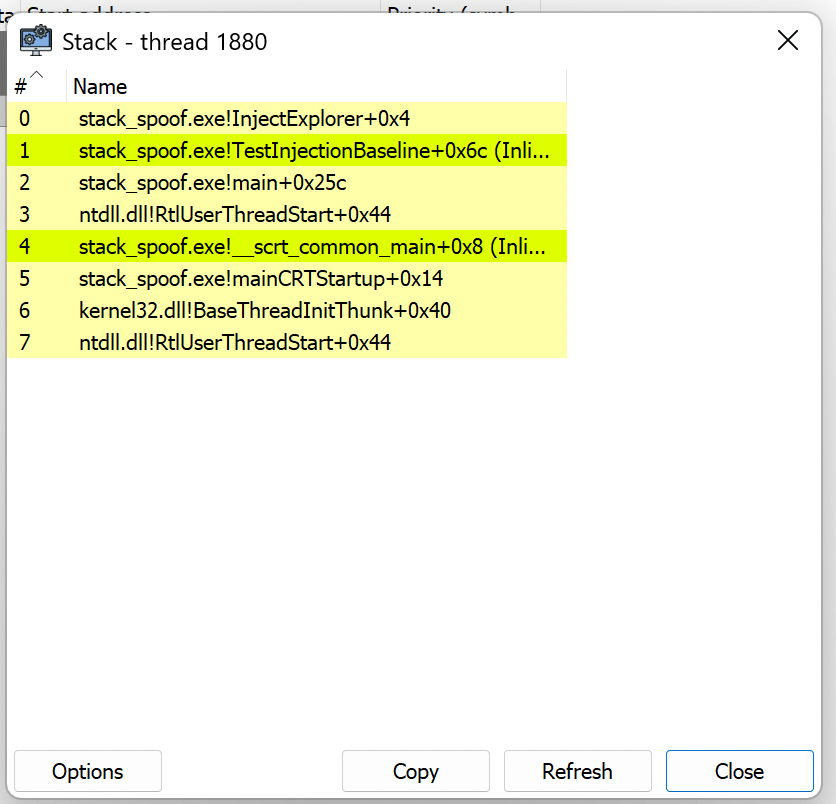
\includegraphics[width=0.72\linewidth]{../artifacts/scenario1/systeminformer-stack.png}
  \caption{System Informer — stack del thread principale con WinDbg in pausa
           su \texttt{InjectExplorer} (Scenario 1). Le righe in giallo
           indicano funzioni inlinate prive di frame proprio.}
  \label{fig:sc1-si}
\end{figure}

\subsection{Riepilogo}

\begin{description}
  \item[CBT (catena \texttt{x29}/\texttt{x30})] 4 frame — catena integra.
        \texttt{TestInjectionBaseline} assente: inlinata da \texttt{/O2},
        nessun frame \texttt{x29} proprio.
  \item[WinDbg / System Informer (\texttt{.pdata})] 9 / 8 frame — vista
        completa tramite unwind virtuale; inline functions visibili come tali.
  \item[SP nei limiti TEB] Sì.
\end{description}

% ── Scenario 2: Single-Frame Spoofing ─────────────────────────────────────────

\section{Scenario 2: Single-Frame Spoofing}
\label{sec:sc2}

Questo scenario introduce la prima tecnica di evasione: un singolo indirizzo di
ritorno falsificato, prelevato da \texttt{ntdll.dll}, viene inserito nella catena
\texttt{x29}/\texttt{x30} in modo che \texttt{CaptureStackBackTrace} lo legga al
posto del vero chiamante.

\subsection{Meccanismo}

Il meccanismo si articola in due fasi distinte:

\begin{enumerate}
  \item \textbf{Gadget discovery.} Il framework scansiona la sezione
        \texttt{.text} di \texttt{ntdll.dll} alla ricerca di istruzioni
        \texttt{BL}. L'indirizzo immediatamente successivo a ciascun
        \texttt{BL} è un \emph{call-site gadget}: un return address valido
        che possiede un record \texttt{RUNTIME\_FUNCTION} in \texttt{.pdata}
        e appartiene a una funzione legittima di sistema.
        In questo run sono stati scoperti 512 gadget (ntdll base
        \texttt{0x00007FFE81EF0000}); il gadget selezionato è
        \texttt{RtlWnfDllUnloadCallback+0x1DFC}
        (\texttt{0x00007FFE\,81EF881C}).

  \item \textbf{Frame falso.} \texttt{SpoofCallStack} costruisce sullo stack
        una struttura \texttt{(FP\_falso, LR\_falso)}: il LR falso è il
        gadget ntdll, il FP falso punta al frame reale di
        \texttt{SpoofCallStack}. Il registro \texttt{x29} viene aggiornato
        per puntare a questa struttura.
\end{enumerate}

\subsection{Codice Rilevante}

\lstinputlisting[style=cstyle, language=C,
  caption={Chiamata a \texttt{SpoofCallStack} con gadget ntdll (Scenario 2).},
  label={lst:sc2-call}]{listings/sc2-spoof-call.c}

\lstinputlisting[style=asmstyle, language=ARM64,
  caption={Implementazione ASM di \texttt{SpoofCallStack}: costruzione del
           frame falso e allocazione secondaria non documentata in
           \texttt{.pdata}.},
  label={lst:sc2-asm}]{listings/sc2-spoof-asm.asm}

\subsection{Stack in Memoria}

SP al breakpoint: \texttt{0x00000056\,9c2ffdf0}.

\begin{table}[H]
\centering
\begin{tabular}{lll}
\toprule
Offset da SP & Valore & Significato \\
\midrule
\texttt{+0x20} & \texttt{0x00000056\,9c2ffe20} & FP del frame falso (frame reale di \texttt{SpoofCallStack}) \\
\texttt{+0x28} & \texttt{0x00007ffe\,81ef72b4} & LR del frame falso = gadget ntdll \\
\texttt{+0x30} & \texttt{0x00000056\,9c2ffef0} & FP reale (frame del chiamante) \\
\texttt{+0x38} & \texttt{0x00007ff6\,c040ce04} & LR reale (indirizzo di ritorno in \texttt{stack\_spoof.exe}) \\
\bottomrule
\end{tabular}
\caption{Dump \texttt{dq sp L10} al breakpoint su \texttt{InjectExplorer}
         (Scenario 2 — Single-Frame Spoofing). Gli offset \texttt{+0x20} e
         \texttt{+0x28} corrispondono alla struttura costruita dal passo~[3]
         del Listato~\ref{lst:sc2-asm}.}
\label{tab:sc2-stack}
\end{table}

{\sloppy SP è all'interno dei limiti TEB
(\texttt{StackBase} \texttt{0x00000056\,9c300000},
\texttt{StackLimit} \texttt{0x00000056\,9c2fb000}).\par}

\subsection{Evidenze Raccolte}

\begin{lstlisting}[style=outstyle,
  caption={\texttt{CaptureStackBackTrace} dall'interno di \texttt{InjectExplorer}
           (Scenario 2 — Single-Frame Spoofing, dati da console)},
  label={lst:sc2-cbt}]
[00] InjectExplorer                           + 0x0060 <-- TARGET
[01] RtlWnfDllUnloadCallback                  + 0x1DFC <-- GADGET
[02] main                                     + 0x03B4
[03] mainCRTStartup                           + 0x0014
[04] BaseThreadInitThunk                      + 0x0040
[05] RtlUserThreadStart                       + 0x0044
\end{lstlisting}

La CBT restituisce 6 frame. Il gadget ntdll è visibile al frame \texttt{[01]}:
\texttt{SpoofCallStack} ha sostituito il LR originale, quindi
\texttt{CaptureStackBackTrace} riporta \texttt{ntdll} come primo chiamante di
\texttt{InjectExplorer}. Tuttavia l'evasione è \emph{parziale}: lo stub
\texttt{SpoofCallStack} (scritto in ASM) esegue un prologo canonico con
\texttt{stp x29, x30} e \texttt{mov x29, sp}, costruendo un frame \texttt{x29}
reale. Il walker CBT risale attraverso questo frame e trova \texttt{main}
al frame \texttt{[02]}: l'attribuzione a \texttt{stack\_spoof.exe} rimane
visibile.

\begin{lstlisting}[style=outstyle,
  caption={Output di \texttt{k} in WinDbg al breakpoint su
           \texttt{InjectExplorer} (Scenario 2 — Single-Frame Spoofing)},
  label={lst:sc2-k}]
 # Child-SP          RetAddr               Call Site
00 00000056`9c2ffdf0 00007ff6`c0401400     stack_spoof!InjectExplorer
01 00000056`9c2ffdf0 00000000`00000000     stack_spoof!SpoofCallStack+0x50
\end{lstlisting}

WinDbg restituisce 2 frame e un \texttt{RetAddr} nullo. Il walker
\texttt{.pdata} risolve il frame di \texttt{InjectExplorer}, poi applica
gli unwind codes di \texttt{SpoofCallStack}: il record \texttt{.pdata} di
\texttt{SpoofCallStack} copre solo il prologo canonico (\texttt{sub sp, sp, \#0x40}),
ma lo stub esegue poi una seconda decremento non documentato
(\texttt{sub sp, sp, \#0x30}). Il walker virtuale non può ricostruire questo
stato, trova un \texttt{RetAddr} nullo e interrompe la traversata.

\begin{figure}[H]
  \centering
  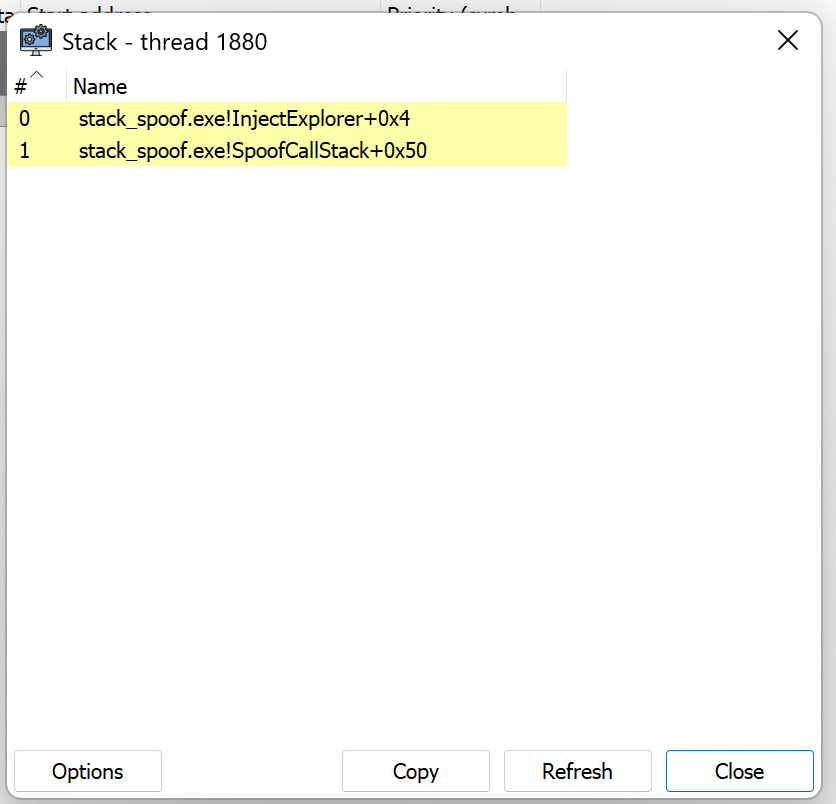
\includegraphics[width=0.72\linewidth]{../artifacts/scenario2/systeminformer-stack.png}
  \caption{System Informer — Scenario 2. Solo 2 frame visibili, entrambi
           evidenziati in giallo: la catena è troncata dopo
           \texttt{SpoofCallStack}. Confrontare con la
           Figura~\ref{fig:sc1-si} (Baseline, 8 frame).}
  \label{fig:sc2-si}
\end{figure}

\subsection{Riepilogo}

\begin{description}
  \item[CBT (catena \texttt{x29}/\texttt{x30})] 6 frame — gadget ntdll
        visibile a \texttt{[01]}, ma \texttt{main} visibile a \texttt{[02]}:
        evasione parziale, attribuzione a \texttt{stack\_spoof.exe} non
        completamente nascosta.
  \item[WinDbg / System Informer (\texttt{.pdata})] 2 frame — catena troncata
        per allocazione secondaria \texttt{-0x30} non documentata in
        \texttt{.pdata}; \texttt{RetAddr} nullo.
  \item[SP nei limiti TEB] Sì.
\end{description}

% ── Scenario 3: Multi-Frame Chain Spoofing ────────────────────────────────────

\section{Scenario 3: Multi-Frame Chain Spoofing}
\label{sec:sc3}

Questo scenario estende la tecnica del Single-Frame Spoofing costruendo una
catena di frame genuini con indirizzi di ritorno falsificati su più livelli.
\texttt{SpoofCallStack} è invocato a tutti e tre i livelli della ricorsione,
incluso il caso base: ogni frame reale di \texttt{RecursiveSpoofHelper} ha il
proprio LR sostituito da un gadget ntdll dedicato.

\subsection{Meccanismo}

\texttt{RecursiveSpoofHelper} si chiama ricorsivamente per 2 livelli prima del
caso base (\texttt{maxDepth} = 2), producendo 3 invocazioni di
\texttt{SpoofCallStack} e 3 gadget ntdll distinti. Poiché ogni frame di
\texttt{RecursiveSpoofHelper} è un frame \texttt{x29} reale (con record
\texttt{.pdata} proprio), la sequenza gadget/frame\allowbreak{}reale che ne risulta è
\emph{strutturalmente valida} dal punto di vista del walker della catena FP.

In questo run sono stati selezionati i seguenti gadget (ntdll base
\texttt{0x00007FFE81EF0000}):

\begin{itemize}
  \item \texttt{Frame[0]}: \texttt{RtlWow64GetProcessMachines+0xA4}
        (\texttt{0x00007FFE\,81EF55E4})
  \item \texttt{Frame[1]}: \texttt{LdrControlFlowGuardEnforced+0x14C}
        (\texttt{0x00007FFE\,81EF449C})
  \item \texttt{Frame[2]} (caso base): \texttt{LdrControlFlowGuardEnforced+0x964}
        (\texttt{0x00007FFE\,81EF4CB4})
\end{itemize}

\subsection{Codice Rilevante}

\lstinputlisting[style=cstyle, language=C,
  caption={\texttt{RECURSIVE\_SPOOF\_CONTEXT} e \texttt{RecursiveSpoofHelper}:
           contesto di ricorsione e sostituzione LR per livello.},
  label={lst:sc3-helper}]{listings/sc3-recursive-helper.c}

Il primitivo \texttt{SpoofCallStack} impiegato ad ogni livello è identico
a quello di Scenario~2 (Listato~\ref{lst:sc2-asm}): la struttura ASM,
l'allocazione secondaria non documentata in \texttt{.pdata} e il gadget ntdll
come LR falso sono invariati.

\subsection{Stack in Memoria}

SP al breakpoint: \texttt{0x00000056\,9c2ffaa0} — inferiore di circa
\texttt{0x350} byte rispetto allo Scenario~2 (\texttt{0x9c2ffdf0}): la
ricorsione a 3 livelli consuma stack aggiuntivo per i frame di
\texttt{RecursiveSpoofHelper} e le allocazioni secondarie di ogni
\texttt{SpoofCallStack}.

\begin{table}[H]
\centering
\begin{tabular}{lll}
\toprule
Offset da SP & Valore & Significato \\
\midrule
\texttt{+0x28} & \texttt{0x00007ffe\,81ef6798} & Gadget ntdll caso base
        (\texttt{LdrControlFlowGuardEnforced}) \\
\texttt{+0x38} & \texttt{0x00007ff6\,c040bc50} & \texttt{RecursiveSpoofHelper}
        in \texttt{stack\_spoof.exe} \\
\texttt{+0x48} & \texttt{0x00007ffe\,81efac40} & Gadget ntdll livello 0
        (\texttt{RtlWow64GetProcessMachines}) \\
\bottomrule
\end{tabular}
\caption{Selezione da \texttt{dq sp L10} al breakpoint su
         \texttt{InjectExplorer} (Scenario 3). Più indirizzi ntdll sono
         visibili nel dump grezzo, intercalati agli indirizzi di
         \texttt{RecursiveSpoofHelper}: struttura ricorsiva leggibile a livello
         raw ma invisibile al walker \texttt{.pdata}.}
\label{tab:sc3-stack}
\end{table}

{\sloppy SP è all'interno dei limiti TEB
(\texttt{StackBase} \texttt{0x00000056\,9c300000},
\texttt{StackLimit} \texttt{0x00000056\,9c2fb000}).\par}

\subsection{Evidenze Raccolte}

\begin{lstlisting}[style=outstyle,
  caption={\texttt{CaptureStackBackTrace} dall'interno di \texttt{InjectExplorer}
           (Scenario 3 — Multi-Frame, dati da console, ntdll base
           \texttt{0x00007FFE81EF0000})},
  label={lst:sc3-cbt}]
[00] InjectExplorer                           + 0x0060 <-- TARGET
[01] LdrControlFlowGuardEnforced              + 0x0964 <-- GADGET Frame[2] (caso base)
[02] RecursiveSpoofHelper                     + 0x0030
[03] LdrControlFlowGuardEnforced              + 0x014C <-- GADGET Frame[1]
[04] RecursiveSpoofHelper                     + 0x0064
[05] RtlWow64GetProcessMachines               + 0x00A4 <-- GADGET Frame[0]
[06] RecursiveSpoofHelper                     + 0x0064
[07] mainCRTStartup                           + 0x0014
[08] BaseThreadInitThunk                      + 0x0040
[09] RtlUserThreadStart                       + 0x0044
\end{lstlisting}

La CBT restituisce 10 frame con il pattern
gadget/\texttt{RecursiveSpoofHelper} che si ripete per 3 livelli. L'offset
\texttt{+0x0030} al frame \texttt{[02]} individua il caso base (chiamata a
\texttt{SpoofCallStack} via \texttt{BL} al \texttt{+0x2C}); gli offset
\texttt{+0x0064} ai frame \texttt{[04]} e \texttt{[06]} individuano il
caso ricorsivo (chiamata ricorsiva anch'essa via \texttt{BL}). Il pattern è
strutturalmente plausibile: alternanza regolare tra funzioni ntdll e funzioni
del binario analizzato. La difficoltà di rilevamento è superiore allo
Scenario~2, dove un singolo gadget ntdll isolato è più evidente.

\begin{lstlisting}[style=outstyle,
  caption={Output di \texttt{k} in WinDbg al breakpoint su
           \texttt{InjectExplorer} (Scenario 3 — Multi-Frame Chain Spoofing)},
  label={lst:sc3-k}]
 # Child-SP          RetAddr               Call Site
00 00000056`9c2ffaa0 00007ff6`c0401400     stack_spoof!InjectExplorer
01 00000056`9c2ffaa0 00000000`00000000     stack_spoof!SpoofCallStack+0x50
\end{lstlisting}

Il dato più rilevante è l'identità tra questo output e quello dello
Scenario~2 (Listato~\ref{lst:sc2-k}). Il walker \texttt{.pdata} raggiunge
\texttt{SpoofCallStack+0x50} e si ferma per lo stesso motivo: l'allocazione
secondaria \texttt{sub sp, sp, \#0x30} non documentata. Il numero di livelli
ricorsivi è completamente invisibile al walker: 1 frame falsificato o 3 sono
indistinguibili dal solo output \texttt{k}. \texttt{RecursiveSpoofHelper}
non compare mai.

\begin{figure}[H]
  \centering
  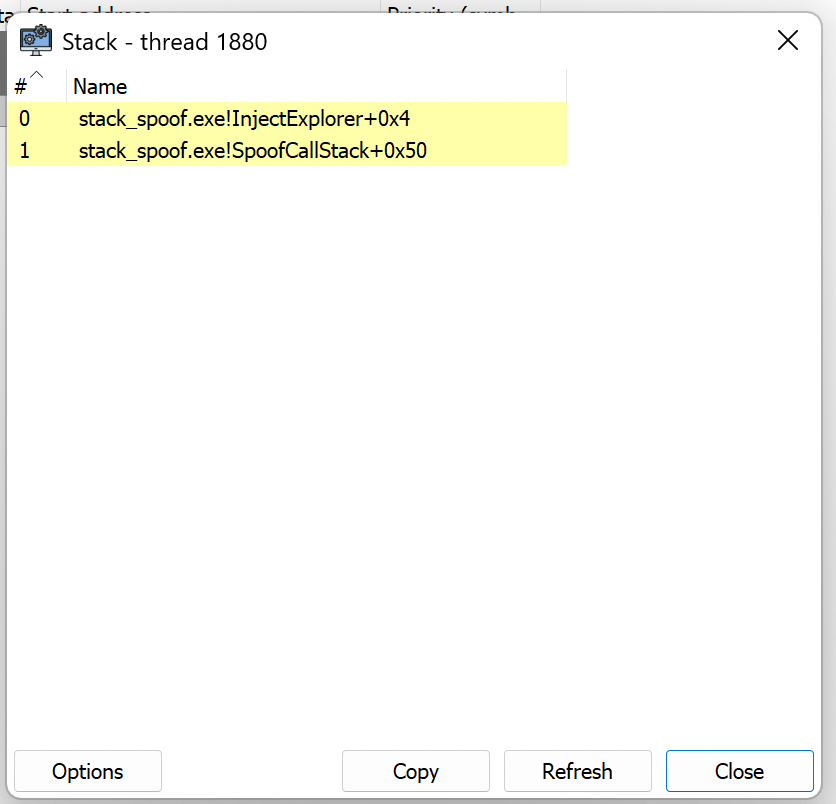
\includegraphics[width=0.72\linewidth]{../artifacts/scenario3/systeminformer-stack.png}
  \caption{System Informer — Scenario 3. Solo 2 frame visibili, entrambi in
           giallo: comportamento identico allo Scenario~2.
           La profondità della catena falsificata è invisibile al walker
           ibrido FP/\texttt{.pdata}.}
  \label{fig:sc3-si}
\end{figure}

\subsection{Riepilogo}

\begin{description}
  \item[CBT (catena \texttt{x29}/\texttt{x30})] 10 frame — pattern
        gadget/frame-reale interleaved strutturalmente valido;
        \texttt{RecursiveSpoofHelper} visibile ma con LR falsificati.
        Attribuzione a \texttt{stack\_spoof.exe} parzialmente visibile
        (frame \texttt{[02][04][06]}), ma più difficile da leggere rispetto
        allo Scenario~2.
  \item[WinDbg / SI (\texttt{.pdata})] 2 frame — \emph{identico} allo
        Scenario~2. Il walker non distingue la profondità della catena
        ricorsiva: 1 o 3 livelli di \texttt{SpoofCallStack} producono lo
        stesso output.
  \item[SP nei limiti TEB] Sì — invariante critico: la struttura è
        indistinguibile da codice legittimo per qualsiasi controllo di bounds.
\end{description}

% ── Scenario 4: Stack Pivot ───────────────────────────────────────────────────

\section{Scenario 4: Stack Pivot}
\label{sec:sc4}

Gli scenari precedenti manipolavano il contenuto dello stack del thread
conservando SP all'interno dei limiti TEB. Questo scenario introduce una
rottura qualitativa: SP viene spostato su una regione di memoria completamente
separata, allocata con \texttt{VirtualAlloc}, invisibile al Thread Environment
Block. Ogni stack walker che validi SP contro
\texttt{[StackLimit, StackBase]} si ferma immediatamente.

\subsection{Meccanismo}

Il primitivo \texttt{ExecuteWithFakeFrame} (Listato~\ref{lst:sc4-asm})
implementa il pivot in quattro fasi:

\begin{enumerate}
  \item \textbf{Salvataggio su stack reale.} Il prologo standard salva tutti
        i registri callee-saved (inclusi \texttt{x29}/\texttt{x30}) sullo
        stack del thread. L'SP reale viene conservato in \texttt{x19},
        l'FP reale in \texttt{x20}, il LR reale in \texttt{x24}.

  \item \textbf{Caricamento del contesto falso.} I tre campi della struttura
        \texttt{FAKE\_FRAME\_DATA} (Listato~\ref{lst:sc4-setup}) sono
        caricati nei registri: \texttt{fakeFp}~\textrightarrow~\texttt{x25},
        \texttt{fakeLr}~\textrightarrow~\texttt{x26} (gadget ntdll),
        \texttt{fakeSp}~\textrightarrow~\texttt{x27} (top del fake stack da
        64~KB allocato con \texttt{VirtualAlloc}).

  \item \textbf{Pivot.} L'istruzione \texttt{mov sp, x27} sposta SP sul fake
        stack. Da questo momento qualsiasi lettura di SP da parte di un
        walker restituisce un indirizzo fuori dall'intervallo TEB. Viene
        costruito un frame (\texttt{sub sp, sp, \#0x20};
        \texttt{stp x25, x26, [sp]}) e \texttt{x29} è aggiornato per
        puntarvi.

  \item \textbf{Chiamata e ripristino.} La funzione target è invocata con
        \texttt{blr x21}; al ritorno, \texttt{mov sp, x19} ripristina lo
        stack reale prima dell'epilogo. L'intera operazione è atomica dal
        punto di vista del chiamante.
\end{enumerate}

\subsection{Codice Rilevante}

\lstinputlisting[style=cstyle, language=C,
  caption={\texttt{FAKE\_FRAME\_DATA} e setup dello Scenario 4: allocazione
           del fake stack e configurazione del pivot.},
  label={lst:sc4-setup}]{listings/sc4-fake-frame-setup.c}

\lstinputlisting[style=asmstyle, language=ARM64,
  caption={Implementazione ASM di \texttt{ExecuteWithFakeFrame}:
           pivot SP verso fake stack, costruzione frame falso,
           ripristino stack reale.},
  label={lst:sc4-asm}]{listings/sc4-execute-fake-frame.asm}

\subsection{Stack in Memoria}

SP al breakpoint: \texttt{0x000001d9\,b4f5ffe0}
(fake stack allocato con \texttt{VirtualAlloc}).

\begin{table}[H]
\centering
\begin{tabular}{lll}
\toprule
Offset da SP & Valore & Significato \\
\midrule
\texttt{+0x00} & \texttt{0x000001d9\,b4f5ff00} & FP falso (entro fake stack) \\
\texttt{+0x08} & \texttt{0x00007ffe\,81ef44e0} & LR falso = gadget ntdll \\
\texttt{+0x10} & \texttt{0x00000000\,00000000} & null \\
\texttt{+0x18} & \texttt{0x00000000\,00000000} & null \\
\texttt{+0x20+} & \texttt{????????\,????????} & oltre il limite di allocazione \\
\bottomrule
\end{tabular}
\caption{Dump \texttt{dq sp L10} al breakpoint su \texttt{InjectExplorer}
         (Scenario 4 — Stack Pivot). SP è sul fake stack: solo 2 quadword
         significativi (FP e LR), poi memoria non allocata.}
\label{tab:sc4-stack}
\end{table}

{\sloppy SP è \textbf{fuori} dai limiti TEB
(\texttt{StackBase} \texttt{0x00000056\,9c300000},
\texttt{StackLimit} \texttt{0x00000056\,9c2fb000}).\par}

\subsection{Evidenze Raccolte}

\begin{lstlisting}[style=outstyle,
  caption={\texttt{CaptureStackBackTrace} dall'interno di \texttt{InjectExplorer}
           (Scenario 4 — Stack Pivot, dati da console)},
  label={lst:sc4-cbt}]
  [STACK TRACE] From inside InjectExplorer (user-mode view):
      (no frames -- stack pivot active)
\end{lstlisting}

La CBT restituisce 0 frame. Prima di percorrere la catena \texttt{x29},
\texttt{CaptureStackBackTrace} verifica che SP sia all'interno dei limiti
TEB (\texttt{x18+0x010} $\leq$ SP $<$ \texttt{x18+0x008}). Poiché SP è sul
fake stack, fuori dall'intervallo \texttt{[StackLimit, StackBase]}, il walker
abortisce prima della prima lettura.

\begin{lstlisting}[style=outstyle,
  caption={Output di \texttt{k} in WinDbg al breakpoint su
           \texttt{InjectExplorer} (Scenario 4 — Stack Pivot)},
  label={lst:sc4-k}]
WARNING: Stack pointer is outside the normal stack bounds.
         Stack unwinding can be inaccurate.
 # Child-SP          RetAddr               Call Site
00 000001d9`b4f5ffe0 00007ff6`c0401564     stack_spoof!InjectExplorer
01 000001d9`b4f5ffe0 00000000`00000000     stack_spoof!ExecuteWithFakeFrame+0x54
\end{lstlisting}

WinDbg emette il \texttt{WARNING} prima di procedere: SP è fuori dai limiti
TEB. Il walker \texttt{.pdata} riesce a risolvere \texttt{InjectExplorer} e
\texttt{ExecuteWithFakeFrame} (entrambi hanno record \texttt{.pdata} validi),
ma trova \texttt{RetAddr} nullo al secondo frame e interrompe la traversata.
La firma residua è inequivocabile: il \texttt{WARNING} stesso è un segnale
di rilevamento.

\begin{figure}[H]
  \centering
  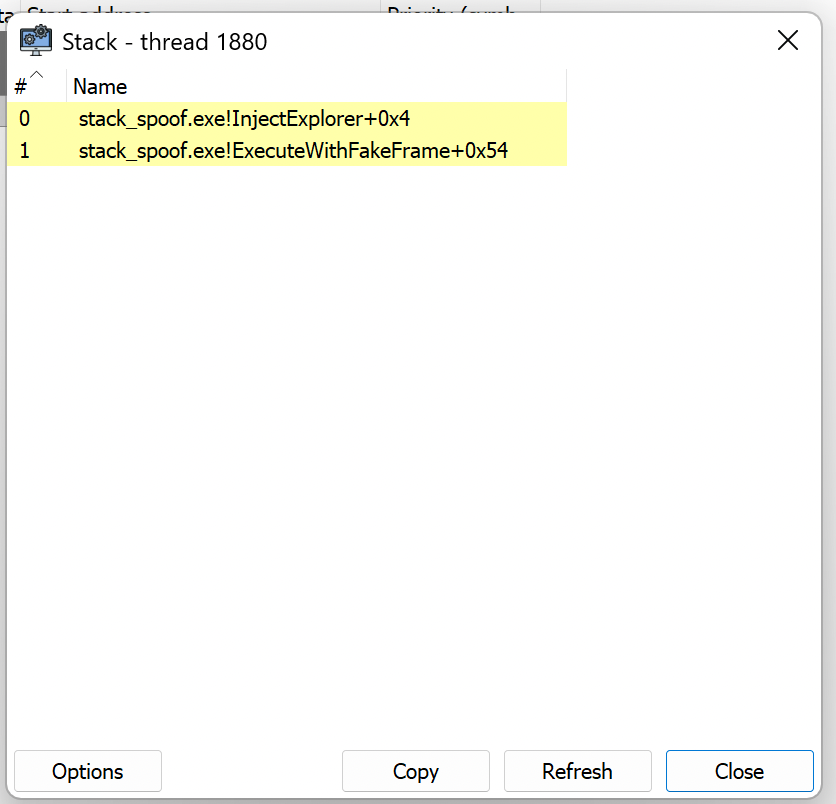
\includegraphics[width=0.72\linewidth]{../artifacts/scenario4/systeminformer-stack.png}
  \caption{System Informer — Scenario 4. 2 frame in giallo:
           \texttt{InjectExplorer} e \texttt{ExecuteWithFakeFrame+0x54}.
           La catena si tronca identicamente a WinDbg.}
  \label{fig:sc4-si}
\end{figure}

\subsection{Riepilogo}

\begin{description}
  \item[CBT (catena \texttt{x29}/\texttt{x30})] 0 frame — SP fuori da
        \texttt{[StackLimit, StackBase]}: il walker abortisce prima della
        prima lettura.
  \item[WinDbg / SI (\texttt{.pdata})] 2 frame con
        \texttt{WARNING: Stack pointer is outside the normal stack bounds}.
        \texttt{ExecuteWithFakeFrame} visibile; firma SP inequivocabile.
  \item[SP nei limiti TEB] No — fake stack allocato con
        \texttt{VirtualAlloc}, range completamente separato dalla stack
        del thread.
\end{description}

% ── Riepilogo Comparativo ─────────────────────────────────────────────────────

\section{Riepilogo Comparativo}
\label{sec:riepilogo-scenari}

La Tabella~\ref{tab:riepilogo} sintetizza le evidenze raccolte per i 4
scenari nei confronti dei 3 strumenti di analisi.

\begin{table}[H]
\centering
\begin{tabular}{lp{3.5cm}p{3.5cm}p{3.5cm}}
\toprule
Scenario & CBT & WinDbg \texttt{k} & System Informer \\
\midrule
1 — Baseline &
  4 frame (catena integra, \texttt{TestInjectionBaseline} inlinata) &
  9 frame completi; inline functions visibili come tali &
  8 frame; funzioni inlinate in giallo \\
\midrule
2 — Single-Frame &
  6 frame; gadget ntdll a \texttt{[01]}, \texttt{main} visibile a \texttt{[02]} &
  2 frame + \texttt{RetAddr} null; \texttt{SpoofCallStack} visibile &
  2 frame gialli \\
\midrule
3 — Multi-Frame &
  10 frame; pattern gadget/\texttt{RSH} $\times$ 3; attribuzione parziale &
  2 frame + \texttt{RetAddr} null; \emph{identico} allo Scenario~2 &
  2 frame gialli \\
\midrule
4 — Stack Pivot &
  0 frame (SP fuori TEB: walker abortisce) &
  \texttt{WARNING} + 2 frame + \texttt{RetAddr} null &
  2 frame gialli \\
\bottomrule
\end{tabular}
\caption{Confronto degli output dei 3 strumenti di analisi per i 4 scenari.
         Il finding chiave dello Scenario~3 è l'identità con lo Scenario~2
         nell'output WinDbg: il walker \texttt{.pdata} non distingue 1 da 3
         livelli di \texttt{SpoofCallStack}. Il finding chiave dello
         Scenario~4 è il \texttt{WARNING} SP: firma residua rilevabile
         anche senza interpretare la call chain.}
\label{tab:riepilogo}
\end{table}

Il dato più significativo dell'analisi comparativa è la \emph{divergenza
strutturale} tra CBT e WinDbg negli Scenari~2 e~3. CBT percorre la catena
\texttt{x29}/\texttt{x30} e riporta fedelmente tutto ciò che trova,
gadget inclusi, ma non può nascondere i frame reali di
\texttt{stack\_spoof.exe} (in particolare \texttt{main}). WinDbg, più
sofisticato nel meccanismo di unwinding, viene ingannato dall'allocazione
secondaria non documentata in \texttt{.pdata}: si ferma a 2 frame in
entrambi gli scenari.

Lo Scenario~3 è il caso più difficile da rilevare in user-mode: SP è nei
limiti TEB, la catena CBT è strutturalmente plausibile (alternanza
regolare funzioni-sistema/funzioni-binario), e il walker \texttt{.pdata}
non distingue la profondità della catena falsificata. Lo Scenario~4 offre
la massima evasione rispetto a CBT (0 frame), ma la firma SP è rilevabile
da qualsiasi strumento che legga i campi TEB, indipendentemente dalla
capacità di interpretare la call chain.
